%%%%%%%%%%%%%%%%%%%%%%%%%%%%%%%%%%%%%%%%%%%%%%%%%%%%%%%%%%%%%%%%%%%%%%%%
%                                                                      %
%     File: Thesis_Control.tex                                         %
%     Tex Master: Thesis.tex                                           %
%                                                                      %
%     Author: Andre C. Marta                                           %
%     Last modified :  05 Aug 2026                                     %
%                                                                      %
%%%%%%%%%%%%%%%%%%%%%%%%%%%%%%%%%%%%%%%%%%%%%%%%%%%%%%%%%%%%%%%%%%%%%%%%

\chapter{System Control}
\label{chapter:control}

Having established, in Chapter~\ref{chapter:modeling}, the kinematic and dynamic models governing the USV and UAV, the natural next step is to determine how these models can be exploited to compute the control inputs that drive each vehicle along a desired trajectory. Because the two vehicles are physically coupled through the tether, their motion cannot be planned independently without accounting for this interaction, motivating a cooperative control strategy.

The overall control approach is therefore established first, followed by the design of the controllers for each vehicle.

\section{Cooperative Control Design}
\label{sec:ctrl_architecture}
Before formulating either controller, the strategies available are weighed against the system's dynamics and its objectives, so that the method chosen suits both vehicles.

\subsection{Control Method}
\label{sec:ctrl_method}

Keeping the tether within safe operating conditions depends on how the distance between the two vehicles evolves over time. A controller that only reacts to the current state can correct a violation only after it happens. Anticipating where the system is headed allows corrective action before reaching the safety limits.

A predictive controller does this by repeatedly solving, at each control instant, an optimization problem over a finite look-ahead window. Because the optimization runs over the predicted trajectory rather than the current state alone, requirements such as keeping the tether within safe conditions can be stated as explicit constraints in the problem itself, enforcing them explicitly over the prediction horizon.

The predictions rely on the model of the system dynamics, so their accuracy is tied to how well that model represents the real behaviour. The USV and UAV models derived in Chapter~\ref{chapter:modeling} include nonlinear terms. The predictive controller uses these nonlinear models directly, making \gls{nmpc} the method used for both vehicles.


\subsection{Cooperative Architecture}
\label{sec:ctrl_coop_architecture}

The USV and the UAV operate on different timescales. The \gls{usv} moves in the horizontal plane with slow, inertia-dominated motion. The \gls{uav}'s dynamics evolve much faster and demand a finer sampling time. A single \gls{nmpc} built around the combined state of both vehicles would force one prediction horizon and one sampling time onto both, compromising one vehicle's timescale to accommodate the other.

Combining both vehicles into one \gls{nmpc} also enlarges the state, input, and constraint sets a single solver must handle, raising the computational cost of a problem that is already time-critical. Keeping the two problems separate matches each optimization's size to its own vehicle and keeps the real-time computation manageable.

Each vehicle is therefore controlled by its own \gls{nmpc}. This separation isolates the two controllers from each other's failures: if one solver fails to find a feasible solution, the other vehicle's \gls{nmpc} continues operating on its own well-posed problem.

The tether's safety limits depend on the relative position between the USV and the UAV, so each vehicle's \gls{nmpc} accounts for the other vehicle's position. At every control instant, each controller receives the other vehicle's predicted position over the prediction horizon and uses it to compute the predicted tether distance at every step of its own horizon. Because the two controllers operate at different sampling intervals, the received predicted trajectory is temporally interpolated and resampled at the receiver's own prediction nodes.

Without this exchange, a vehicle would have to treat the other as stationary or extrapolate its motion from the last known state. Either assumption misrepresents the tether coupling and can drive the system into a constraint violation.

Figure~\ref{fig:ctrl_architecture} shows this architecture, with two independent \gls{nmpc} loops, each driving its own vehicle, exchanging predicted horizons to enforce the tether constraint.

\begin{figure}[H]
    \centering
    \definecolor{okiBlue}{rgb}{0.0,0.447,0.698}
    \definecolor{okiGreen}{rgb}{0.0,0.620,0.451}
    \definecolor{okiVermillion}{rgb}{0.835,0.369,0.0}

    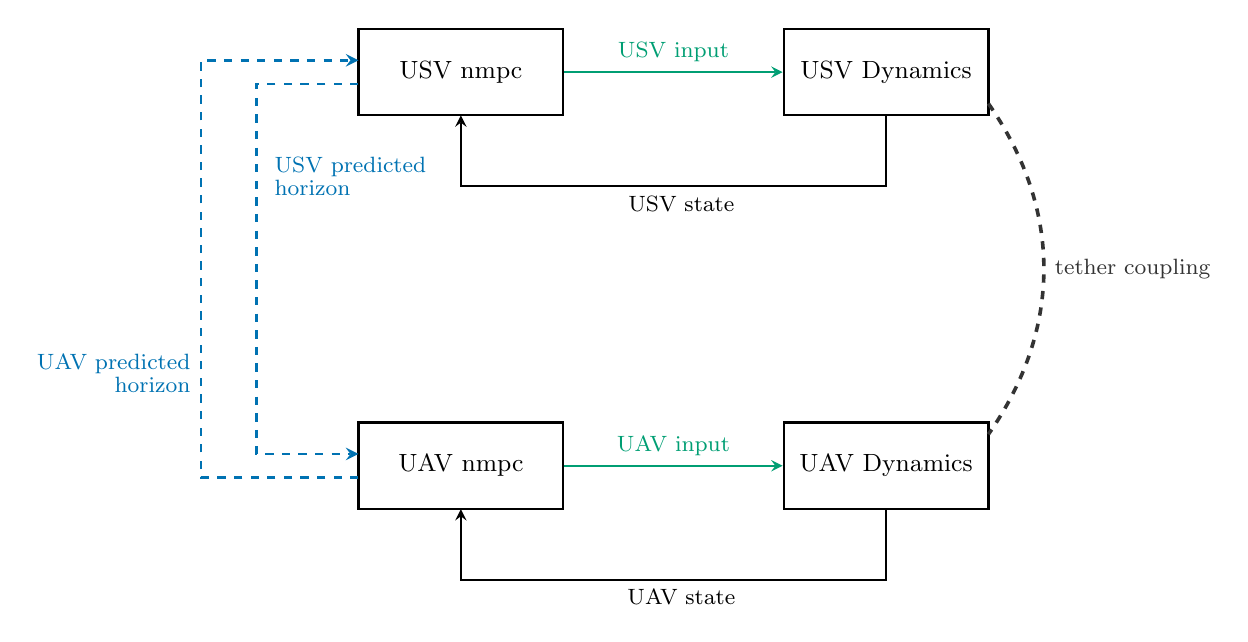
\begin{tikzpicture}[
        >=stealth,
        every node/.style={font=\small},
        boxStyle/.style={draw, rectangle, minimum height=1.1cm, minimum width=2.6cm, align=center, thick},
        sigArrow/.style={->, black, thick},
        exArrow/.style={->, okiBlue, dashed, line width=1.0pt},
        tetherStyle/.style={black!80, dashed, line width=1.3pt}
    ]

        % ---------- USV loop (top) ----------
        \node[boxStyle] (usvnmpc) at (0,5) {USV \gls{nmpc}};
        \node[boxStyle] (usvplant) at (5.4,5) {USV Dynamics};

        \draw[->, okiGreen, thick] (usvnmpc) -- (usvplant)
            node[midway, above, font=\footnotesize] {USV input};

        \draw[sigArrow] (5.4,4.45) -- (5.4,3.55) -- (0,3.55) -- (0,4.45);
        \node[below, font=\footnotesize] at (2.8,3.55) {USV state};

        % ---------- UAV loop (bottom) ----------
        \node[boxStyle] (uavnmpc) at (0,0) {UAV \gls{nmpc}};
        \node[boxStyle] (uavplant) at (5.4,0) {UAV Dynamics};

        \draw[->, okiGreen, thick] (uavnmpc) -- (uavplant)
            node[midway, above, font=\footnotesize] {UAV input};

        \draw[sigArrow] (5.4,-0.55) -- (5.4,-1.45) -- (0,-1.45) -- (0,-0.55);
        \node[below, font=\footnotesize] at (2.8,-1.45) {UAV state};

        % ---------- Coordination exchange between the two NMPCs ----------
        \draw[exArrow] (-1.3,4.85) -- (-2.6,4.85) -- (-2.6,0.15)
            node[pos=0.25, right, align=left, font=\footnotesize, xshift=0.1cm]
            {USV predicted\\[-1pt] horizon}
            -- (-1.3,0.15);

        \draw[exArrow] (-1.3,-0.15) -- (-3.3,-0.15) -- (-3.3,5.15)
            node[pos=0.25, left, align=right, font=\footnotesize]
            {UAV predicted\\[-1pt] horizon}
            -- (-1.3,5.15);

        % ---------- Physical tether coupling between plants ----------
        \draw[tetherStyle] (6.7,4.6) to[bend left=35]
            node[midway, right, font=\footnotesize] {tether coupling} (6.7,0.4);

    \end{tikzpicture}
    \caption{Cooperative control architecture diagram.}
    \label{fig:ctrl_architecture}
\end{figure}

\section{Nonlinear Model Predictive Control}
\label{sec:ctrl_nmpc_principles}

The vehicle models of Chapter~\ref{chapter:modeling} are continuous-time systems of the form
\begin{equation}
    \dot{\mathbf{x}} = \mathbf{f}\left( \mathbf{x}, \mathbf{u} \right),
    \label{eq:nmpc_dynamics_continuous}
\end{equation}
where $\mathbf{x} \in \mathbb{R}^{n_x}$ is the state vector and $\mathbf{u} \in \mathbb{R}^{n_u}$ is the control input vector. Since the controller acts at discrete sampling instants $t_k = k T_s$, with the input held constant over each interval $[t_k, t_{k+1})$, the exact system state evolves as
\begin{equation}
    \mathbf{x}(t_{k+1}) = \mathbf{x}_k + \int_{t_k}^{t_{k+1}} \mathbf{f}\left( \mathbf{x}(\tau), \mathbf{u}_k \right) d\tau \approx \boldsymbol\Phi\left( \mathbf{x}_k, \mathbf{u}_k \right),
    \label{eq:nmpc_dynamics_general}
\end{equation}
where the one-step discrete map $\boldsymbol\Phi$ numerically approximates this integral over $T_s$. \gls{nmpc} computes, at every instant $k$, the input that steers this system toward a reference over a finite look-ahead window of $N$ steps.

At instant $k$, denote by $\hat{\mathbf{x}}_{k+i|k}$ and $\hat{\mathbf{u}}_{k+i|k}$ the state and input predicted $i$ steps ahead, for $i = 0, \dots, N$. The hat marks a predicted quantity rather than the true system state. The predicted trajectory starts from the current measured or estimated state,
\begin{equation}
    \hat{\mathbf{x}}_{k|k} = \mathbf{x}_k,
    \label{eq:nmpc_x0}
\end{equation}
and evolves according to the system model,
\begin{equation}
    \hat{\mathbf{x}}_{k+i+1|k} = \boldsymbol\Phi\left( \hat{\mathbf{x}}_{k+i|k}, \hat{\mathbf{u}}_{k+i|k} \right), \quad i = 0, \dots, N-1.
    \label{eq:nmpc_prediction}
\end{equation}

Each predicted step is then scored against a reference trajectory. A stage cost $\ell(\hat{\mathbf{x}}_{k+i|k}, \hat{\mathbf{u}}_{k+i|k})$ penalizes the tracking error and the control effort at every step of the horizon, and a terminal cost $\ell_f(\hat{\mathbf{x}}_{k+N|k})$ penalizes the tracking error at its final step. Summing both over the horizon gives the total predicted cost,
\begin{equation}
    J = \sum_{i=0}^{N-1} \ell\left( \hat{\mathbf{x}}_{k+i|k}, \hat{\mathbf{u}}_{k+i|k} \right) + \ell_f\left( \hat{\mathbf{x}}_{k+N|k} \right).
    \label{eq:nmpc_cost}
\end{equation}

Minimizing $J$ alone ignores the physical limits of the system, so the prediction is also constrained. Direct bounds apply to the state and the input at every step of the horizon,
\begin{align}
    \hat{\mathbf{x}}_{k+i|k} &\in \mathcal{X}, \quad i = 0, \dots, N, \label{eq:nmpc_bounds_x} \\
    \hat{\mathbf{u}}_{k+i|k} &\in \mathcal{U}, \quad i = 0, \dots, N-1, \label{eq:nmpc_bounds_u}
\end{align}
where $\mathcal{X}$ and $\mathcal{U}$ collect the admissible states and inputs. Additional requirements that combine state and input, or that cannot be expressed as simple bounds, are stated as a general path constraint,
\begin{equation}
    \mathbf{g}\left( \hat{\mathbf{x}}_{k+i|k}, \hat{\mathbf{u}}_{k+i|k} \right) \le \mathbf{0}, \quad i = 0, \dots, N-1.
    \label{eq:nmpc_path_constraint}
\end{equation}
Pure state constraints, such as geometric workspace boundaries, naturally extend to the terminal node as well, taking the form $\mathbf{g}_N\left(\hat{\mathbf{x}}_{k+N|k}\right) \le \mathbf{0}$.

Assembling the cost, the prediction model, and the constraints defines the optimal control problem solved at every sampling instant $k$:
\begin{align}
    \min_{\hat{\mathbf{x}}_{k+i|k}, \, \hat{\mathbf{u}}_{k+i|k}} \quad & J \label{eq:nmpc_ocp_cost} \\
    \text{s.t.} \quad & \hat{\mathbf{x}}_{k|k} = \mathbf{x}_k, \notag \\
    & \hat{\mathbf{x}}_{k+i+1|k} = \boldsymbol\Phi\left( \hat{\mathbf{x}}_{k+i|k}, \hat{\mathbf{u}}_{k+i|k} \right), \quad i = 0, \dots, N-1, \notag \\
    & \hat{\mathbf{x}}_{k+i|k} \in \mathcal{X}, \quad i = 0, \dots, N, \notag \\
    & \hat{\mathbf{u}}_{k+i|k} \in \mathcal{U}, \quad i = 0, \dots, N-1, \notag \\
    & \mathbf{g}\left( \hat{\mathbf{x}}_{k+i|k}, \hat{\mathbf{u}}_{k+i|k} \right) \le \mathbf{0}, \quad i = 0, \dots, N-1, \notag \\
    & \mathbf{g}_N\left( \hat{\mathbf{x}}_{k+N|k} \right) \le \mathbf{0}. \notag
\end{align}

Solving this problem returns a full predicted input sequence, $\hat{\mathbf{u}}_{k|k}, \dots, \hat{\mathbf{u}}_{k+N-1|k}$, but only its first element, $\hat{\mathbf{u}}_{k|k}$, is applied to the system. At the next instant, $k+1$, the state is measured again and the problem is solved from scratch, now anchored at $\hat{\mathbf{x}}_{k+1|k+1}$. Under the receding horizon principle, the horizon slides forward with time, and every applied input comes from a fresh optimization over the current prediction, not from a plan fixed in advance.


\section{USV NMPC}
\label{sec:ctrl_usv_mpc}

The USV NMPC computes, at every sampling instant, the thruster commands that best track a reference trajectory over a finite prediction horizon, subject to the vessel's dynamics, the physical limits of its actuators, and the tether workspace. It predicts the vessel's motion with the model derived in Chapter~\ref{chapter:modeling}, and solves a constrained optimization problem at each step to obtain the commands applied to the thrusters.

\subsubsection*{Predictive Model}

The input $\mathbf{u}_v = [X,Y,N]^\top$ of the vessel model is the resultant thrust force and moment, obtained from the physical actuator commands $T_L, T_R, \alpha_L, \alpha_R$ through the allocation
\begin{equation}
    X = T_L\cos\alpha_L + T_R\cos\alpha_R, \qquad Y = T_L\sin\alpha_L + T_R\sin\alpha_R,
    \label{eq:usv_mpc_alloc_force}
\end{equation}
\begin{equation}
    N = -x_{arm}\big(T_L\sin\alpha_L+T_R\sin\alpha_R\big) - y_{arm}\big(T_L\cos\alpha_L-T_R\cos\alpha_R\big).
    \label{eq:usv_mpc_alloc_moment}
\end{equation}
Since the controller's ultimate goal is always to command $T_L, T_R, \alpha_L, \alpha_R$, the most direct approach is to let the NMPC choose them itself, redefining the input vector as $\mathbf{u}_v = [T_L, T_R, \alpha_L, \alpha_R]^\top$ rather than choosing $X,Y,N$ and allocating separately. This also guarantees that every value chosen by the NMPC is attainable, since the bounds are imposed directly on the physical actuator commands, rather than on an approximation of their combined effect.

However, the thrusters can only change thrust and azimuth at a limited rate,
\begin{equation}
    \mathcal{U}: \; |\dot{T}_L| \le \dot{T}_{L,max}, \quad |\dot{T}_R| \le \dot{T}_{R,max}, \quad |\dot{\alpha}_L| \le \dot{\alpha}_{L,max}, \quad |\dot{\alpha}_R| \le \dot{\alpha}_{R,max}.
    \label{eq:usv_mpc_input_bounds}
\end{equation}
To impose \eqref{eq:usv_mpc_input_bounds} directly, $T_L, T_R, \alpha_L, \alpha_R$ are treated as states rather than as inputs,
\begin{equation}
    \mathbf{x}_v = [x, y, \psi, u, v, r,\ T_L, T_R, \alpha_L, \alpha_R]^\top \in \mathbb{R}^{10}.
    \label{eq:usv_mpc_state_augmented}
\end{equation}
Their time derivative is then used as the control input,
\begin{equation}
    \mathbf{u}_v = [\dot{T}_L, \dot{T}_R, \dot{\alpha}_L, \dot{\alpha}_R]^\top \in \mathbb{R}^4,
    \label{eq:usv_mpc_input_augmented}
\end{equation}
so that the rate limits in \eqref{eq:usv_mpc_input_bounds} become direct bounds on $\mathbf{u}_v$.

With $\mathbf{x}_v$ and $\mathbf{u}_v$ defined, the dynamics $\dot{\mathbf{x}}_v = \mathbf{f}_v(\mathbf{x}_v,\mathbf{u}_v)$ follow directly.

The kinematics are given by \eqref{eq:usv_kinematics_planar} and \eqref{eq:usv_psi_dot},
\begin{equation}
    \dot x = u\cos\psi - v\sin\psi, \qquad \dot y = u\sin\psi + v\cos\psi, \qquad \dot\psi = r.
    \label{eq:usv_mpc_kinematics}
\end{equation}

The dynamics follow \eqref{eq:usv_udot}--\eqref{eq:usv_rdot}, with $X,Y,N$ given by \eqref{eq:usv_mpc_alloc_force}--\eqref{eq:usv_mpc_alloc_moment} in terms of the thruster state,
\begin{equation}
    \dot u = \frac{1}{m}\Big[X - \big(X_u+X_{uu}^{\pm}|u|\big)u\Big] + vr,
    \label{eq:usv_mpc_udot}
\end{equation}
\begin{equation}
    \dot v = \frac{1}{m}\Big[Y - \big(Y_v+Y_{vv}|v|\big)v\Big] - ur,
    \label{eq:usv_mpc_vdot}
\end{equation}
\begin{equation}
    \dot r = \frac{1}{I_z}\Big[N - \big(N_r+N_{rr}|r|\big)r\Big].
    \label{eq:usv_mpc_rdot}
\end{equation}

Finally, $\dot T_L,\dot T_R,\dot\alpha_L,\dot\alpha_R$ appear directly as the components of $\mathbf{u}_v$,
\begin{equation}
    \dot T_L = \dot T_L, \qquad \dot T_R = \dot T_R, \qquad \dot\alpha_L = \dot\alpha_L, \qquad \dot\alpha_R = \dot\alpha_R.
    \label{eq:usv_mpc_thruster_rates}
\end{equation}

Discretization over a sampling interval $T_s$, following Section~\ref{sec:ctrl_nmpc_principles}, gives the one-step map $\boldsymbol\Phi_v$ such that $\hat{\mathbf{x}}_{v,k+i+1|k} = \boldsymbol\Phi_v\big(\hat{\mathbf{x}}_{v,k+i|k}, \hat{\mathbf{u}}_{v,k+i|k}\big)$ approximates the solution of $\dot{\mathbf{x}}_v = \mathbf{f}_v(\mathbf{x}_v,\mathbf{u}_v)$ over one sampling interval.


\subsubsection*{Cost and Constraints}
 
Let $\mathbf{p} = [x,y]^\top$ and $\boldsymbol{\nu} = [u,v,r]^\top$ denote the position and body-fixed velocities, and $\psi$ the heading, with $\mathbf{p}_{ref}$, $\psi_{ref}$, and $\boldsymbol{\nu}_{ref}$ the corresponding references.

Tracking the reference position is penalized as
\begin{equation}
    \|\mathbf{p}-\mathbf{p}_{ref}\|^2_{Q_p},
    \label{eq:usv_mpc_cost_pos}
\end{equation}
where $\|\boldsymbol\xi\|^2_W \coloneqq \boldsymbol\xi^\top W \boldsymbol\xi$ for a positive semi-definite weighting matrix $W$, which sets the relative importance of each component of $\boldsymbol\xi$ in the cost.

Tracking the heading reference is penalized as
\begin{equation}
    q_\psi\big(1-\cos(\psi-\psi_{ref})\big).
    \label{eq:usv_mpc_cost_heading}
\end{equation}
Both $\psi$ and $\psi_{ref}$ are angles represented within an interval of width $2\pi$, such as $(-\pi,\pi]$. When they lie near opposite ends of this interval, their raw difference $\psi-\psi_{ref}$ approaches $\pm2\pi$, even though the two headings are then almost identical. As $\cos(\cdot)$ has period exactly $2\pi$, $\cos(\psi-\psi_{ref})$ evaluates to exactly the same value whether $\psi-\psi_{ref}$ is close to $0$ or close to $\pm2\pi$, so \eqref{eq:usv_mpc_cost_heading} correctly assigns a similarly small cost in both cases.

Tracking the reference velocity is penalized in the same way as the position,
\begin{equation}
    \|\boldsymbol{\nu}-\boldsymbol{\nu}_{ref}\|^2_{Q_\nu}.
    \label{eq:usv_mpc_cost_vel}
\end{equation}

The thruster commands $T_L, T_R, \alpha_L, \alpha_R$ are regularized directly as
\begin{equation}
    \big\|[T_L,T_R,\alpha_L,\alpha_R]^\top\big\|^2_{Q_\tau},
    \label{eq:usv_mpc_cost_reg}
\end{equation}
discouraging thrust and azimuth commands larger than necessary to track the reference. Unlike the UAV in hover, where a non-zero thrust is strictly required at rest to counteract gravity, the vessel at rest ($\boldsymbol{\nu} = \mathbf{0}$) is in unforced equilibrium. While penalizing thrust toward zero slightly counteracts the thrust required to overcome hydrodynamic drag at cruising speed, this trade-off is balanced by choosing $Q_\tau \ll Q_\nu$, ensuring negligible steady-state speed tracking error.

The last term penalizes $\mathbf{u}_v$, the rate of change of the thruster commands,
\begin{equation}
    \big\|[\dot{T}_L, \dot{T}_R, \dot{\alpha}_L, \dot{\alpha}_R]^\top\big\|^2_{R} = \|\mathbf{u}_v\|^2_{R},
    \label{eq:usv_mpc_cost_rate}
\end{equation}
discouraging abrupt changes in thrust and azimuth between consecutive instants.

Summing \eqref{eq:usv_mpc_cost_pos}--\eqref{eq:usv_mpc_cost_rate} gives the stage cost
\begin{equation}
    \begin{aligned}
        \ell(\mathbf{x}_v, \mathbf{u}_v) = {} & \|\mathbf{p}-\mathbf{p}_{ref}\|^2_{Q_p} + q_\psi\big(1-\cos(\psi-\psi_{ref})\big) + \|\boldsymbol{\nu}-\boldsymbol{\nu}_{ref}\|^2_{Q_\nu} \\
        & + \big\|[T_L,T_R,\alpha_L,\alpha_R]^\top\big\|^2_{Q_\tau} + \|\mathbf{u}_v\|^2_{R}.
    \end{aligned}
    \label{eq:usv_mpc_stage_cost}
\end{equation}

The terminal cost $\ell_f$ penalizes the tracking and state regularization errors of the last predicted state, preventing the finite horizon from letting them grow unchecked near its end. It preserves the tracking and actuator state regularization terms of \eqref{eq:usv_mpc_stage_cost} and drops only the input rate penalty $\|\mathbf{u}_v\|^2_R$, since no control input is chosen at the final node of the horizon:
\begin{equation}
    \ell_f(\mathbf{x}_v) = \|\mathbf{p}-\mathbf{p}_{ref}\|^2_{Q_p} + q_\psi\big(1-\cos(\psi-\psi_{ref})\big) + \|\boldsymbol{\nu}-\boldsymbol{\nu}_{ref}\|^2_{Q_\nu} + \big\|[T_L,T_R,\alpha_L,\alpha_R]^\top\big\|^2_{Q_\tau}.
    \label{eq:usv_mpc_terminal_cost}
\end{equation}
 
Each thruster is physically limited in the values $T_L, T_R, \alpha_L, \alpha_R$ can take. Since these commands are components of $\mathbf{x}_v$, this defines the admissible state set
\begin{equation}
    \mathcal{X}: \; T_{L,min} \le T_L \le T_{L,max}, \;\; T_{R,min} \le T_R \le T_{R,max}, \;\; \alpha_{L,min} \le \alpha_L \le \alpha_{L,max}, \;\; \alpha_{R,min} \le \alpha_R \le \alpha_{R,max}.
    \label{eq:usv_mpc_state_bounds}
\end{equation}

The tether also couples the vessel to the UAV, requiring the distance between the vessel deck attachment point and the drone to remain within the maximum admissible separation distance $d_{max}$. At every sampling instant, the USV controller receives the UAV's predicted trajectory $\hat{\mathbf{p}}_a = [\hat x_a, \hat y_a, \hat z_a]^\top$ over the prediction horizon, temporally resampled at the vessel's prediction nodes. This geometric constraint is formulated as
\begin{equation}
    h_v(\mathbf{x}_v) = (x - \hat x_a)^2 + (y - \hat y_a)^2 + \hat z_a^2 - d_{max}^2 \le \sigma_v,
    \label{eq:usv_mpc_tether_constraint}
\end{equation}
where $\sigma_v \ge 0$ is a non-negative slack variable that softens the boundary to prevent solver infeasibility under external disturbances. The slack is penalized in the cost through
\begin{equation}
    \rho_v(\sigma_v) = \mu_{1,v}\sigma_v + \mu_{2,v}\sigma_v^2, \qquad \mu_{1,v}, \mu_{2,v} \ge 0,
    \label{eq:usv_mpc_slack_penalty}
\end{equation}
with large weights $(\mu_{1,v}, \mu_{2,v})$ ensuring that violations are kept close to zero whenever geometrically feasible.
 
\subsubsection*{Optimal Control Problem}
 
At every sampling instant $k$, the kinematic and dynamic components of the initial state come from the vessel's current estimate, while the thruster components use the last command actually applied:
\begin{equation}
    \mathbf{x}_{v,0} = \big[x_k, y_k, \psi_k, u_k, v_k, r_k,\ T_{L,k-1}, T_{R,k-1}, \alpha_{L,k-1}, \alpha_{R,k-1}\big]^\top.
    \label{eq:usv_mpc_initial_condition}
\end{equation}
This ensures that the first step of the horizon already departs from the actuators' true state, and therefore respects the rate limits in \eqref{eq:usv_mpc_input_bounds} from the very first input chosen.
 
Assembling the cost, the model, and the constraints gives the optimal control problem the USV solves at every sampling instant:
\begin{align}
    \min_{\hat{\mathbf{x}}_v,\, \hat{\mathbf{u}}_v,\, \hat{\sigma}_v} \quad & \sum_{i=0}^{N-1} \Big[\ell\big(\hat{\mathbf{x}}_{v,k+i|k}, \hat{\mathbf{u}}_{v,k+i|k}\big) + \rho_v\big(\hat\sigma_{v,k+i|k}\big)\Big] + \ell_f\big(\hat{\mathbf{x}}_{v,k+N|k}\big) + \rho_v\big(\hat\sigma_{v,k+N|k}\big) \notag \\
    \text{s.t.} \quad & \hat{\mathbf{x}}_{v,k|k} = \mathbf{x}_{v,0}, \notag \\
    & \hat{\mathbf{x}}_{v,k+i+1|k} = \boldsymbol\Phi_v\big(\hat{\mathbf{x}}_{v,k+i|k}, \hat{\mathbf{u}}_{v,k+i|k}\big), \quad i = 0, \dots, N-1, \notag \\
    & \hat{\mathbf{x}}_{v,k+i|k} \in \mathcal{X}, \quad i = 0, \dots, N, \notag \\
    & \hat{\mathbf{u}}_{v,k+i|k} \in \mathcal{U}, \quad i = 0, \dots, N-1, \notag \\
    & h_v\big(\hat{\mathbf{x}}_{v,k+i|k}\big) \le \hat\sigma_{v,k+i|k}, \quad \hat\sigma_{v,k+i|k} \ge 0, \quad i = 0, \dots, N. \label{eq:usv_mpc_ocp}
\end{align}
The vessel's low-level actuators receive the integrated thruster commands $T_{L,k}, T_{R,k}, \alpha_{L,k}, \alpha_{R,k}$ obtained by integrating the first optimal input rate $\hat{\mathbf{u}}_{v,k|k}$ over the sampling interval $T_s$. These become the thruster components of the initial state at the subsequent sampling instant.
 
%%%%%%%%%%%%%%%%%%%%%%%%%%%%%%%%%%%%%%%%%%%%%%%%%%%%%%%%%%%%%%%%%%%%%%%%%%%%%%%%%%%%%%%%%
\section{UAV NMPC}
\label{sec:ctrl_uav_mpc}

The UAV NMPC computes, at every sampling instant, the thrust and attitude commands that best track a reference trajectory relative to the vessel over a finite prediction horizon, subject to the vehicle's dynamics, its actuation limits, and the tether workspace. It predicts the vehicle's motion with the model derived in Chapter~\ref{chapter:modeling}, and solves a constrained optimization problem at each step to obtain the commands applied to the vehicle.

\subsubsection*{Predictive Model}

The input $\mathbf{u}_a = [T,\phi,\theta,\psi]^\top$ of the vehicle model defined in Chapter~\ref{chapter:modeling} commands the thrust and the attitude directly, assuming each of them is reached instantaneously.

Similarly to the thruster commands of the USV, the attitude $\phi,\theta,\psi$ is limited in how fast it can change. To constrain these rates directly, $\phi,\theta,\psi$ are treated here as states rather than as the input,
\begin{equation}
    \mathbf{x}_a = [x,y,z,\dot x,\dot y,\dot z,\ \phi,\theta,\psi]^\top \in \mathbb{R}^{9}.
    \label{eq:uav_mpc_state_augmented}
\end{equation}
Their time derivative is then used as the input, so that the rate constraint applies to it directly,
\begin{equation}
    \mathbf{u}_a = [\dot\phi,\dot\theta,\dot\psi,T]^\top \in \mathbb{R}^4.
    \label{eq:uav_mpc_input_augmented}
\end{equation}

With $\mathbf{x}_a$ and $\mathbf{u}_a$ defined, the dynamics $\dot{\mathbf{x}}_a = \mathbf{f}_a(\mathbf{x}_a,\mathbf{u}_a)$ follow directly.

The kinematics are the trivial identity already used in \eqref{eq:uav_kinematics},
\begin{equation}
    \dot x = \dot x, \qquad \dot y = \dot y, \qquad \dot z = \dot z.
    \label{eq:uav_mpc_kinematics}
\end{equation}

The translational dynamics follow \eqref{eq:uav_dynamics}, with the thrust term expanded and the tether force $\mathbf{F}_{\mathrm{tether}}^{\mathcal{I}} = [F_{\mathrm{tether},x}^{\mathcal{I}}, F_{\mathrm{tether},y}^{\mathcal{I}}, F_{\mathrm{tether},z}^{\mathcal{I}}]^\top$ given by \eqref{eq:uav_tether_geometry}--\eqref{eq:uav_tether_force},
\begin{equation}
    \ddot x = \frac{T}{m}\big(\cos\psi\sin\theta\cos\phi+\sin\psi\sin\phi\big) + \frac{1}{m}F_{\mathrm{tether},x}^{\mathcal{I}},
    \label{eq:uav_mpc_xddot}
\end{equation}
\begin{equation}
    \ddot y = \frac{T}{m}\big(\sin\psi\sin\theta\cos\phi-\cos\psi\sin\phi\big) + \frac{1}{m}F_{\mathrm{tether},y}^{\mathcal{I}},
    \label{eq:uav_mpc_yddot}
\end{equation}
\begin{equation}
    \ddot z = \frac{T}{m}\cos\theta\cos\phi - g + \frac{1}{m}F_{\mathrm{tether},z}^{\mathcal{I}}.
    \label{eq:uav_mpc_zddot}
\end{equation}

Finally, $\dot\phi,\dot\theta,\dot\psi$ appear directly as the first three components of $\mathbf{u}_a$,
\begin{equation}
    \dot\phi = \dot\phi, \qquad \dot\theta = \dot\theta, \qquad \dot\psi = \dot\psi.
    \label{eq:uav_mpc_attitude_rates}
\end{equation}

Discretization over a sampling interval $T_s$, following Section~\ref{sec:ctrl_nmpc_principles}, gives the one-step map $\boldsymbol\Phi_a$ such that $\hat{\mathbf{x}}_{a,k+i+1|k} = \boldsymbol\Phi_a\big(\hat{\mathbf{x}}_{a,k+i|k},\hat{\mathbf{u}}_{a,k+i|k}\big)$ approximates the solution of $\dot{\mathbf{x}}_a = \mathbf{f}_a(\mathbf{x}_a,\mathbf{u}_a)$ over one sampling interval.

\subsubsection*{Cost and Constraints}

Let $\mathbf{p} = [x,y,z]^\top$ and $\mathbf{v} = [\dot x,\dot y,\dot z]^\top$ denote the position and velocity, with $\mathbf{p}_{ref}$ and $\mathbf{v}_{ref}$ the corresponding references.

Tracking the reference position and velocity is penalized as
\begin{equation}
    \|\mathbf{p}-\mathbf{p}_{ref}\|^2_{Q_p} + \|\mathbf{v}-\mathbf{v}_{ref}\|^2_{Q_v}.
    \label{eq:uav_mpc_cost_track}
\end{equation}

The next term penalizes $\phi,\theta$ directly, rather than comparing them against any reference,
\begin{equation}
    \big\|[\phi,\theta]^\top\big\|^2_{Q_{tilt}},
    \label{eq:uav_mpc_cost_tilt}
\end{equation}
discouraging attitude larger than necessary to track the reference.

The next term penalizes the yaw error, but rather than tracking a fixed yaw angle, $\psi$ is aligned with the direction to a reference point $\mathbf{p}_{b,ref} = [x_{b,ref},y_{b,ref}]^\top$, itself possibly varying along the horizon,
\begin{equation}
    \mathbf{b} = \mathbf{p}_{b,ref} - \mathbf{p}_{xy},
    \label{eq:uav_mpc_yaw_direction}
\end{equation}
where $\mathbf{p}_{xy}=[x,y]^\top$. Since $\psi$ is an angle, the same periodicity used in \eqref{eq:usv_mpc_cost_heading} applies, expressed here as an alignment between $\psi$ and the bearing vector $\mathbf{b}$ rather than a difference between two angles,
\begin{equation}
    q_\psi\left(1 - \frac{\cos\psi\,b_x + \sin\psi\,b_y}{\|\mathbf{b}\|}\right).
    \label{eq:uav_mpc_cost_yaw}
\end{equation}
This term is minimized when $\psi$ points along $\mathbf{b}$, the direction to the reference point $\mathbf{p}_{b,ref}$.

The last term penalizes the input $\mathbf{u}_a$. Penalizing $T$ toward zero would fight the physics of hover, where thrust must counteract gravity rather than vanish. To keep this term a measure of control effort rather than a penalty on the thrust needed just to hover, the input is tracked against a reference $\mathbf{u}_{a,ref} = [0,0,0,mg]^\top$, using $mg$ as a nominal hover approximation,
\begin{equation}
    \|\mathbf{u}_a - \mathbf{u}_{a,ref}\|^2_{R},
    \label{eq:uav_mpc_cost_input}
\end{equation}
so that $\dot\phi,\dot\theta,\dot\psi$ are regularized toward zero, while $T$ is penalized only for deviating from this nominal hover value.

Summing the tracking, tilt, yaw, and input penalties in \eqref{eq:uav_mpc_cost_track}, \eqref{eq:uav_mpc_cost_tilt}, \eqref{eq:uav_mpc_cost_yaw}, and \eqref{eq:uav_mpc_cost_input} gives the stage cost
\begin{equation}
    \begin{aligned}
        \ell(\mathbf{x}_a,\mathbf{u}_a) = {} & \|\mathbf{p}-\mathbf{p}_{ref}\|^2_{Q_p} + \|\mathbf{v}-\mathbf{v}_{ref}\|^2_{Q_v} + \big\|[\phi,\theta]^\top\big\|^2_{Q_{tilt}} \\
        & + q_\psi\left(1 - \frac{\cos\psi\,b_x + \sin\psi\,b_y}{\|\mathbf{b}\|}\right) + \|\mathbf{u}_a-\mathbf{u}_{a,ref}\|^2_R.
    \end{aligned}
    \label{eq:uav_mpc_stage_cost}
\end{equation}

The terminal cost $\ell_f$ keeps the tracking and attitude regularization terms of \eqref{eq:uav_mpc_stage_cost} and drops the input penalty, since no input is chosen at the final node of the horizon:
\begin{equation}
    \begin{aligned}
        \ell_f(\mathbf{x}_a) = {} & \|\mathbf{p}-\mathbf{p}_{ref}\|^2_{Q_p} + \|\mathbf{v}-\mathbf{v}_{ref}\|^2_{Q_v} + \big\|[\phi,\theta]^\top\big\|^2_{Q_{tilt}} \\
        & + q_\psi\left(1 - \frac{\cos\psi\,b_x + \sin\psi\,b_y}{\|\mathbf{b}\|}\right).
    \end{aligned}
    \label{eq:uav_mpc_terminal_cost}
\end{equation}

The vehicle's operating envelope bounds the altitude, translational velocity, and attitude. To guarantee safe clearance above the water surface and vessel deck, the vehicle is restricted to $z \ge z_{min}$. Furthermore, because horizontal and vertical velocities are limited by distinct physical factors, the vehicle's speed and tilt are bounded separately:
\begin{equation}
    z \ge z_{min}, \quad \big\|[\dot x,\dot y]^\top\big\| \le v_{xy,max}, \quad |\dot z| \le v_{z,max}, \quad |\phi| \le \phi_{max}, \quad |\theta| \le \theta_{max}.
    \label{eq:uav_mpc_state_bounds}
\end{equation}

Unlike the thruster commands of the USV, which the previous instant's own command already keeps within their bounds, the velocity and attitude of \eqref{eq:uav_mpc_state_bounds} are subject to external disturbances such as wind. A gust can push the vehicle's true state past these bounds regardless of what the NMPC has commanded, and if they are enforced as hard bounds, the solver has no feasible solution to return from such a state, even though it must still produce one at every sampling instant.

A soft constraint avoids this by allowing a bound to be exceeded, at a cost. Each bound in \eqref{eq:uav_mpc_state_bounds} is loosened by its own slack variable $\sigma_j \ge 0$, $j=1,\dots,5$:
\begin{align}
    z_{min} - z &\le \sigma_1, \label{eq:uav_mpc_slack_z} \\
    \big\|[\dot x,\dot y]^\top\big\| - v_{xy,max} &\le \sigma_2, \label{eq:uav_mpc_slack_vxy} \\
    |\dot z| - v_{z,max} &\le \sigma_3, \label{eq:uav_mpc_slack_vz} \\
    |\phi| - \phi_{max} &\le \sigma_4, \label{eq:uav_mpc_slack_phi} \\
    |\theta| - \theta_{max} &\le \sigma_5. \label{eq:uav_mpc_slack_theta}
\end{align}
Each slack is penalized through the quadratic-linear penalty function
\begin{equation}
    \rho_j(\sigma_j) = \mu_{1,j}\sigma_j + \mu_{2,j}\sigma_j^2, \qquad \mu_{1,j},\mu_{2,j}\ge0,
    \label{eq:uav_mpc_slack_penalty}
\end{equation}
penalizing $\sigma_j>0$ while still preferring $\sigma_j=0$ whenever the original bound can be met on its own.

The attitude rates and the thrust are bounded as hard constraints on the input:
\begin{equation}
    \mathcal{U}: \; |\dot\phi| \le \dot\phi_{max}, \quad |\dot\theta| \le \dot\theta_{max}, \quad |\dot\psi| \le \dot\psi_{max}, \quad T_{min} \le T \le T_{max}.
    \label{eq:uav_mpc_input_bounds}
\end{equation}

The tether limits the distance between the vehicle and its attachment point on the vessel, at position $\mathbf{p}_v = [x_v,y_v,0]^\top$, to the maximum admissible separation distance $d_{max}$. The distance $d_{max}$ is chosen with sufficient margin relative to the total deployed tether length to maintain non-negative slack $\varepsilon \ge 0$. Since the vessel is itself being predicted by the USV NMPC, $\mathbf{p}_v$ is received at each node as the vessel's predicted position there, temporally resampled to match the UAV sampling instants. This geometric constraint is softened with its own slack $\sigma_6\ge0$:
\begin{equation}
    h_a(\mathbf{x}_a) = (x-x_v)^2 + (y-y_v)^2 + z^2 - d_{max}^2 \le \sigma_6,
    \label{eq:uav_mpc_tether_constraint}
\end{equation}
weighted more heavily by \eqref{eq:uav_mpc_slack_penalty} with large parameters $(\mu_{1,6},\mu_{2,6})$, keeping it close to strictly enforced.

Assembling \eqref{eq:uav_mpc_slack_z}--\eqref{eq:uav_mpc_slack_theta} and \eqref{eq:uav_mpc_tether_constraint}, with their slacks stacked as $\boldsymbol\sigma=[\sigma_1,\dots,\sigma_6]^\top\ge\mathbf{0}$, gives the soft constraint set $\mathcal{X}_\sigma$ of admissible pairs $(\mathbf{x}_a,\boldsymbol\sigma)$, and the aggregate penalty
\begin{equation}
    P(\boldsymbol\sigma) = \sum_{j=1}^{6} \rho_j(\sigma_j).
    \label{eq:uav_mpc_aggregate_penalty}
\end{equation}

\subsubsection*{Optimal Control Problem}

At every sampling instant $k$, the initial state is set from the vehicle's current state estimate:
\begin{equation}
    \mathbf{x}_{a,0} = \big[x_k,y_k,z_k,\dot x_k,\dot y_k,\dot z_k,\ \phi_k,\theta_k,\psi_k\big]^\top.
    \label{eq:uav_mpc_initial_condition}
\end{equation}

Assembling the cost, the model, and the constraints gives the optimal control problem the UAV solves at every sampling instant, with the slack vector $\hat{\boldsymbol\sigma}_{k+i|k}$ entering as an additional decision variable:
\begin{align}
    \min_{\hat{\mathbf{x}}_a,\,\hat{\mathbf{u}}_a,\,\hat{\boldsymbol\sigma}} \quad & \sum_{i=0}^{N-1} \Big[\ell\big(\hat{\mathbf{x}}_{a,k+i|k},\hat{\mathbf{u}}_{a,k+i|k}\big) + P\big(\hat{\boldsymbol\sigma}_{k+i|k}\big)\Big] + \ell_f\big(\hat{\mathbf{x}}_{a,k+N|k}\big) + P\big(\hat{\boldsymbol\sigma}_{k+N|k}\big) \notag \\
    \text{s.t.} \quad & \hat{\mathbf{x}}_{a,k|k} = \mathbf{x}_{a,0}, \notag \\
    & \hat{\mathbf{x}}_{a,k+i+1|k} = \boldsymbol\Phi_a\big(\hat{\mathbf{x}}_{a,k+i|k},\hat{\mathbf{u}}_{a,k+i|k}\big), \quad i=0,\dots,N-1, \notag \\
    & \big(\hat{\mathbf{x}}_{a,k+i|k},\hat{\boldsymbol\sigma}_{k+i|k}\big) \in \mathcal{X}_\sigma, \quad i=0,\dots,N, \notag \\
    & \hat{\mathbf{u}}_{a,k+i|k} \in \mathcal{U}, \quad i=0,\dots,N-1. \label{eq:uav_mpc_ocp}
\end{align}
The vehicle's low-level autopilot receives the integrated attitude setpoints and thrust command corresponding to the end of the first sampling interval, obtained by applying the optimal rate input $\hat{\mathbf{u}}_{a,k|k}$ over $T_s$.